\documentclass[10pt]{article}
\usepackage{fullpage}
\usepackage{graphicx}
\usepackage{caption}
\usepackage{url}

\newcommand{\chidb}{$\chi$\textsf{db}}

%opening
\title{The \chidb{} File Format\\{\large Version 0.20100327}}
\author{Borja Sotomayor}
\date{}

\begin{document}
\pagestyle{empty}
\maketitle

\chidb{} is a didactic relational database management system (RDBMS) designed for teaching how a RDBMS is built internally, from the data organization in files all the way up to the SQL parser and query optimizer. The design of \chidb{} is based on SQLite\footnote{\url{http://www.sqlite.org/}}, with several simplifying assumptions that make it possible to develop a complete \chidb{} implementation over the course of a quarter or semester. One of the key similarities is that \chidb{} uses a single file to store all its information (database metadata, tables, and indexes). In fact, the \chidb{} file format is a subset of SQLite, meaning that well-formed \chidb{} files will also be well-formed SQLite files (the converse, though, is not necessarily true).

This document describes the format of a \chidb{} database file. We assume a basic knowledge of RDBMS (a student should know what a table and an index is) and what a B-Tree is. How the file is created and updated (e.g., how to add a new entry to a B-Tree) is outside the scope of this document. 

The format of the file is described in a top-down fashion. The document starts off with an overview of the file format, and then focuses on how tables are stored in it. Since indexes share many common traits (in terms of format) with tables, they are discussed at the end of the document, focusing on the differences with tables. Thus, the document begins with an overview of how a \chidb{} file is organized, both physically and logically, in Section~\ref{sec:overview}, followed by a brief description of supported datatypes in Section~\ref{sec:datatypes} and a description of the file header in Section~\ref{sec:header}. Next, the format of table pages (Section~\ref{sec:tablepages}), table cells (Section~\ref{sec:tablecells}), and database records (Section~\ref{sec:records}) is described. The format of indexes is described in Section~\ref{sec:indexes}. Finally, the format of the schema table, a special table which stores the database schema, is described in Section~\ref{sec:schema}.

\section{File format overview}
\label{sec:overview}

The \chidb{} file format is a subset of the SQLite file format\footnote{\url{http://www.sqlite.org/fileformat.html}} and, thus, shares many common traits with it. A \chidb{} file can store any number of tables, physically stored as a B-Tree, and a table can have records with any number of fields of different datatypes. Indexes are also supported, and also stored as B-Trees. However, \chidb{} makes the following simplifying assumptions:

\begin{itemize}
 \item Each table must have an explicit primary key (SQLite allows tables without primary keys to be created), and the primary key must be a single unsigned 4 byte integer field.
 \item Indexes can only be created for unsigned 4-byte integer unique fields.
 \item Only a subset of the SQLite datatypes are supported.
 \item The size of a record cannot exceed the size of a database page (more specifically, SQLite overflow pages are not supported). This effectively also limits the size of certain datatypes (such as strings).
 \item The current format is geared towards using the database file only for insertion and querying. Although record removal and update are not explicitly disallowed, their implementation cannot be done efficiently in the current format.
 \item A user is assumed to have exclusive access to the database file.
\end{itemize}

These assumptions were made to simplify the implementation of many low-level details, so that students can focus on higher-level ideas (but still requiring a healthy amount of low-level programming). For example, although supporting database records that span multiple pages is a necessary feature in production databases, its implementation requires a fair amount of low-level programming that is algorithmically dull (at least when compared with algorithms for B-Tree insertion, query optimization, etc.).

The remainder of this section provides an overview of the logical organization of a \chidb{} file, followed by its physical organization. Figure~\ref{fig:physlog} summarizes the file organization, and the relationship between logical and physical organization. Specific details (e.g., ``In what part exactly of the database file should I store a B-Tree entry?'') are provided in the next sections.

\begin{figure}
\begin{center}
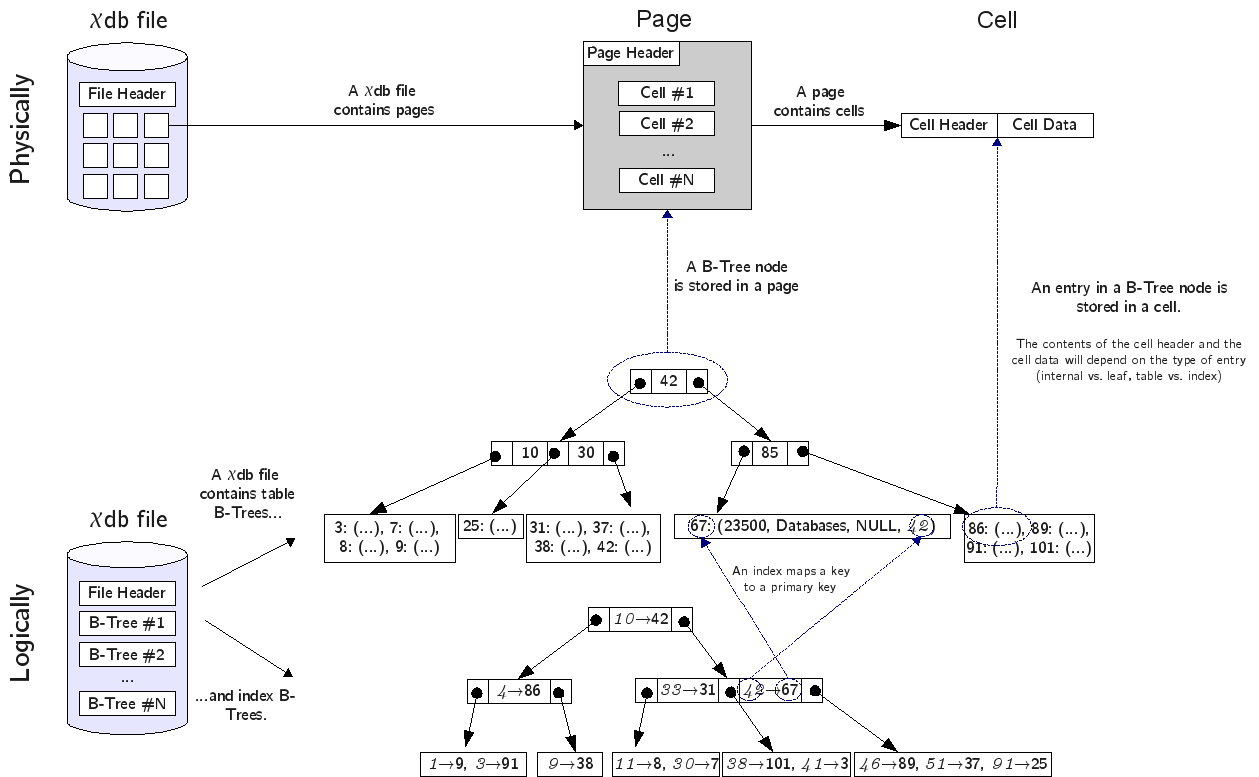
\includegraphics[width=\textwidth]{images/physlog.png}
\caption{Physical and logical file organization}
\end{center}
\label{fig:physlog}
\end{figure}


\subsection{Logical organization}

A \chidb{} file contains the following:

\begin{itemize}
\item[---] A file header.
\item[---] 0 or more tables.
\item[---] 0 or more indexes.
\end{itemize}

The \emph{\textbf{file header}} contains metadata about the database file, most of which is relevant to the physical organization of the file. The file header does \emph{not} contain the database schema (i.e., the specification of tables and indexes in the database), which is stored in a special table called the \emph{schema table} (described in Section~\ref{sec:schema}).

Each \emph{\textbf{table}} in the database file is stored as a B$^+$-Tree (hereafter we will refer to these simply as ``table B-Trees''). The entries of this tree are \emph{\textbf{database records}} (a collection of values corresponding to a row in the table). The key for each entry will be its primary key. Since a table is a B$^+$-tree, the internal nodes do not contain entries but, rather, are used to navigate the tree.

Each \emph{\textbf{index}} in the database file is stored as a B-Tree (hereafter we will refer to these as ``index B-Trees''). Assuming we have a relation $R(pk,\ldots,ik,\ldots)$ where $pk$ is the primary key, and $ik$ is the attribute we want to create an index over, each entry in an index B-Tree will be a $(k_1, k_2)$ pair, where $k_1$ is a value of $ik$ and $k_2$ is the value of the primary key ($pk$) in the record where $ik=k_1$. More formally, using relational algebra:

\[
k_2=\Pi_{pk} \sigma_{ik=k_1} R
\]

The entries are ordered (and thus keyed) by the value of $k_1$. Note that an index B-Tree contains as many entries as the table it indexes. Furthermore, since it is a B-Tree (as opposed to a B$^+$-Tree), both the internal and leaf nodes contain entries (the internal nodes, additionally, include pointers to child nodes).

\subsection{Physical organization}
\label{sec:physorg}

A \chidb{} file is divided into \emph{\textbf{pages}}\footnote{Pages are sometimes referred to as 'blocks' in the literature. They are the units of transfer between secondary storage and memory} of size \textsc{Page--Size}, numbered from 1. Each page is used to store a table or index B-Tree node.

A page contains a \emph{\textbf{page header}} with metadata about the page, such as the type of page (e.g., does it store an internal table node? a leaf index node?). The space not used by the header is available to store \emph{\textbf{cells}}, which are used to store B-Tree entries:

\begin{description}
\item[Leaf Table cell]: $\langle \textsc{Key}, \textsc{DB--Record} \rangle$, where \textsc{DB--Record} is a database record and \textsc{Key} is its primary key.
\item[Internal Table cell]: $\langle \textsc{Key}, \textsc{Child--Page} \rangle$, where \textsc{Child--Page} is the number of the page containing the entries with keys less than or equal to \textsc{Key}.
\item[Leaf Index cell]: $\langle \textsc{Key--Idx}, \textsc{Key--Pk} \rangle$, where \textsc{Key--Idx} and \textsc{Key--Pk} are $k_1$ and $k_2$, respectively, as defined earlier.
\item[Internal Index cell]: $\langle \textsc{Key--Idx}, \textsc{Key--Pk}, \textsc{Child--Page} \rangle$, where \textsc{Key--Idx} and \textsc{Key--Pk} are defined as above, and \textsc{Child--Page} is the number of the page containing the entries with keys less than \textsc{Key--Idx}.
\end{description}

Page 1 in the database is special, as its first 100 bytes are used by the file header. Thus, the B-Tree node stored in page 1 can only use $(\textsc{Page-Size} - 100)$ bytes.

Although the exact format of the page, page header, and cells will be explained later, it is worth explaining one of the values stored in the page header here. First, note how internal cells store a key and a \textsc{Child--Page} ``pointer''\footnote{In the literature, B-Tree nodes are shown as being linked with pointers. It is worth emphasizing that, when storing a B-Tree in a file, this ``pointer'' is simply the number of the page where the referenced node can be found}. However, a B-Tree node must have, by definition, $n$ keys and $n+1$ pointers. Using cells, however, we can only store $n$ pointers. Given a node $B$, an extra pointer is necessary to store the number of the page containing the node $B'$ with keys greater than all the keys in $B$. This extra pointer is stored in the page header and is called \textsc{Right--Page}. Figure~\ref{fig:rightpage} shows a B-Tree both logically and physically. Notice how the \textsc{Right--Page} pointer is, essentially, the ``rightmost pointer'' in a B-Tree node.

\begin{figure}
\begin{center}
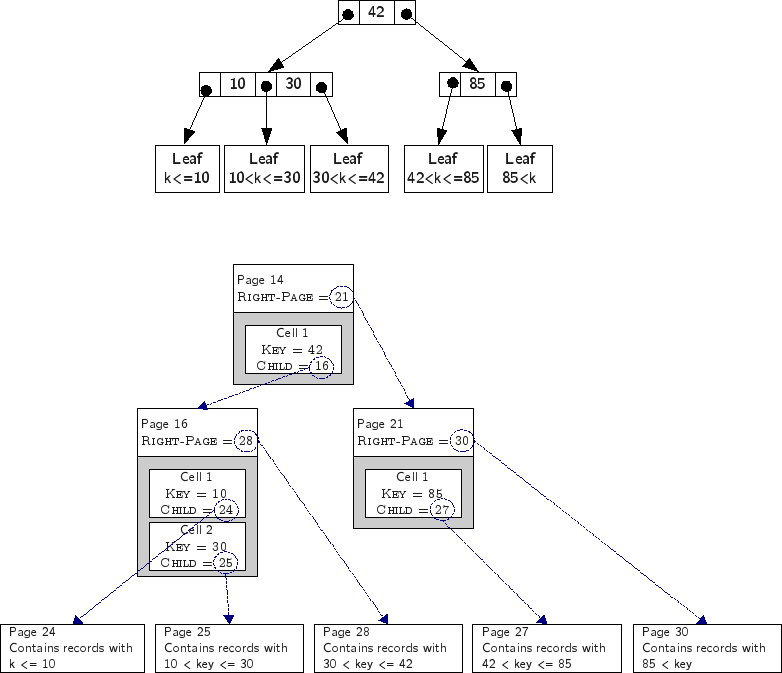
\includegraphics[width=0.8\textwidth]{images/rightpage.png}
\caption{Logical and physical view of a table B-Tree.}
\end{center}
\label{fig:rightpage}
\end{figure}


\section{Datatypes}
\label{sec:datatypes}

\chidb{} uses a limited number of integer and string datatypes, summarized in Table~\ref{tab:datatypes}. All integer types are big-endian. All string types use lower ASCII encoding (or, equivalently, 1-byte UTF-8). Note that these are not the types for the database records (which are described in Section~\ref{sec:records}) but, rather, datatypes used internally in the database file.

\begin{table}
\caption{Datatypes}
\begin{center}
\sffamily
\begin{tabular}{|l|l|l|}
\hline \textbf{Bytes} & \textbf{Name} & \textbf{Range} \\ \hline\hline
\textsf{uint8} & Unsigned 1-byte integer &  $0 \leq x \leq 255$ \\ \hline
\textsf{uint16} & Unsigned 2-byte integer & $0 \leq x \leq 65,535$ \\ \hline
\textsf{uint32} & Unsigned 4-byte integer &  $0 \leq x \leq 2^{32}-1$ \\ \hline
\textsf{int8} & Signed 1-byte integer &  $-128 \leq x \leq 127$\\ \hline
\textsf{int16} & Signed 2-byte integer & $-32768 \leq x \leq 32767$  \\ \hline 
\textsf{int32} & Signed 4-byte integer & $-2^{31} \leq x \leq 2^{31}-1$  \\ \hline
\textsf{varint8} & Unsigned 1-byte varint &  $0 \leq x \leq 127$  \\ \hline
\textsf{varint32} & Unsigned 2-byte varint &  $0 \leq x \leq 2^{28}-1$ \\ \hline
\textsf{string($n$)} & Nul-terminated string & \# of characters $\leq n$ \\\hline
\textsf{raw--string($n$)} & Character array &  \# of characters $\leq n$ \\\hline
\end{tabular}
\end{center}
\label{tab:datatypes}
\end{table}

\textsf{varint} is a special integer type that is supported for compatibility with SQLite. A \textsf{varint} is a variable-length integer encoding that can store a 64-bit signed integer using 1-9 bytes, depending on the value of the integer. To simplify the \chidb{} file format, this datatype is not fully supported. However, since the \textsf{varint} type is essential to the SQLite data format, 1-byte and 4-byte \textsf{varint}s are supported (hereafter referred to as \textsf{varint8}  and \textsf{varint32}, respectively). Note that, in \chidb{}, these are \emph{not} variable length integers; they just follow the format of a variable-length integer encoding in the particular cases when 1 or 4 bytes are used. Thus, whenever this document specifies that a \textsf{varint32} is used, that means that exactly 4 bytes (with the format explained below) will be used. There is no need to determine what the `length' of the integer is.

In a \textsf{varint8}, the most significant bit is always set to \texttt{0}. The remainder of the byte is used to store an unsigned 7-bit integer:

\begin{center}
\texttt{0xxxxxxx}
\end{center}

In a \textsf{varint32}, the most significant bit of the three most significant bytes is always set to \texttt{1} and the most significant bit of the least significant byte is always set to \texttt{0}. The remaining bits are used to store a big-endian unsigned 28-bit integer:

\begin{center}
\texttt{1xxxxxxx 1xxxxxxx 1xxxxxxx 0xxxxxxx}
\end{center}

\section{File header}
\label{sec:header}

The first 100 bytes of a \chidb{} file contain a header with metadata about the file. This file header uses the same format as SQLite and, since many SQLite features are not supported in \chidb{}, most of the header contains constant values. The layout of the header is shown in Figure~\ref{fig:fileheader}. Note that, at this point, all values except \textsc{Page--Size} can be safely ignored, but they must all be properly initialized to the values shown in the table in Figure~\ref{fig:fileheader}.

\begin{figure}
\begin{center}
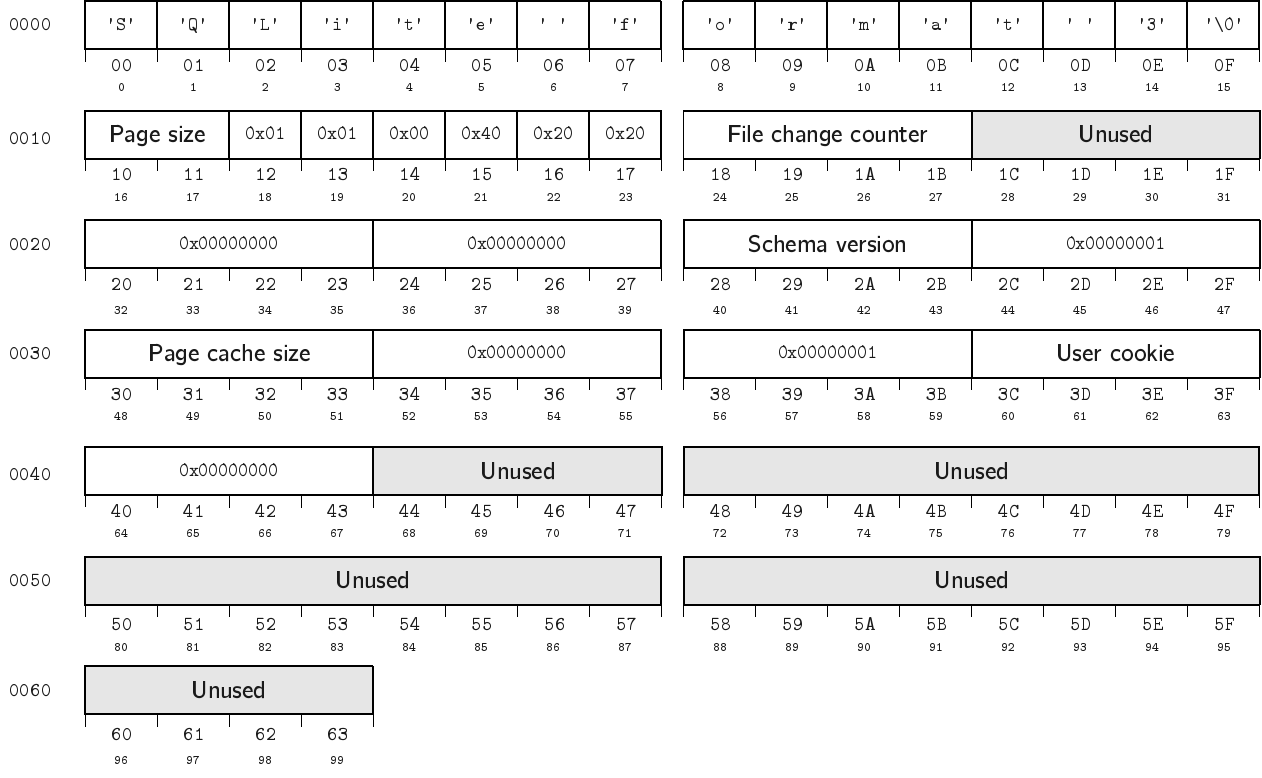
\includegraphics[width=0.8\textwidth]{images/fileheader.png}

\vspace{2em}

\sffamily
\begin{tabular}{|c|c|c|p{7cm}|}
\hline \textbf{Bytes} & \textbf{Name} & \textbf{Type} & {\centering \textbf{Description}} \\ \hline\hline
16-17 & \textsc{Page--Size} & \textsf{uint16} & Size of database page \\ \hline
24-27 & \textsc{File--Change--Counter} & \textsf{uint32}  & Initialized to \texttt{0}. Each time a modification is made to the database, this counter is increased.\\ \hline
40-43 & \textsc{Schema--Version} & \textsf{uint32}  & Initialized to \texttt{0}. Each time the database schema is modified, this counter is increased. \\ \hline
48-51 & \textsc{Page--Cache--Size} & \textsf{uint32}  & Default pager cache size in bytes. Initialized to \texttt{20000}\\\hline
60-43 & \textsc{User--Cookie} & \textsf{uint32}  & Available to the user for read-write access. Initialized to \texttt{0}\\ \hline
\end{tabular}
\caption{\chidb{} file header}
\end{center}
\label{fig:fileheader}
\end{figure}

\section{Table pages}
\label{sec:tablepages}

A table page is composed of four section: the \emph{\textbf{page header}}, the \emph{\textbf{cells}}, the \emph{\textbf{cell offset array}}, and \emph{\textbf{free space}}. To understand how they relate to each other, it is important to understand how cells are laid out in a page. A table page is, to put is simply, a container of cells. The bytes in a page of size \textsc{Page--Size} are numbered from 0 to ($\textsc{Page--Size}-1$). Byte 0 is the \emph{top} of the page, and byte ($\textsc{Page--Size}-1$) is the \emph{bottom} of the page. Cells are stored in a page from the bottom up. For example, if a cell of size $c_1$ is added to an empty page, that cell would occupy bytes ($\textsc{Page--Size}-c_1$) through ($\textsc{Page--Size}-1$). If another cell of size $c_2$ is added, that cell would occupy bytes ($\textsc{Page--Size}-c_1-c_2$) through ($\textsc{Page--Size}-c_1-1$). New cells are always added at the top of the cell area, cells must always be contiguous and there can be no free space between them. Thus, removing a cell or modifying its contents requires instantly defragmenting the cells.

The cell offset array is used to keep track of where each cell is located. The cell offset array is located at the top of the page (after the page header) and grows from the top down. The $i^\textrm{th}$ entry of the array contains the byte offset of the $i^\textrm{th}$ cell \emph{by increasing key order}. In other words, the cell offset is used not only to determine the location of each cell, but also their correct order. Figure~\ref{fig:celloffsetarray} shows an example of how the insertion of a new cells affects the cell offset array. Notice how the new cell is stored at the top of the cell area, regardless of its key value. On the other hand, the entry in the cell offset array for the new cell is inserted in order.

\begin{figure}
\begin{center}
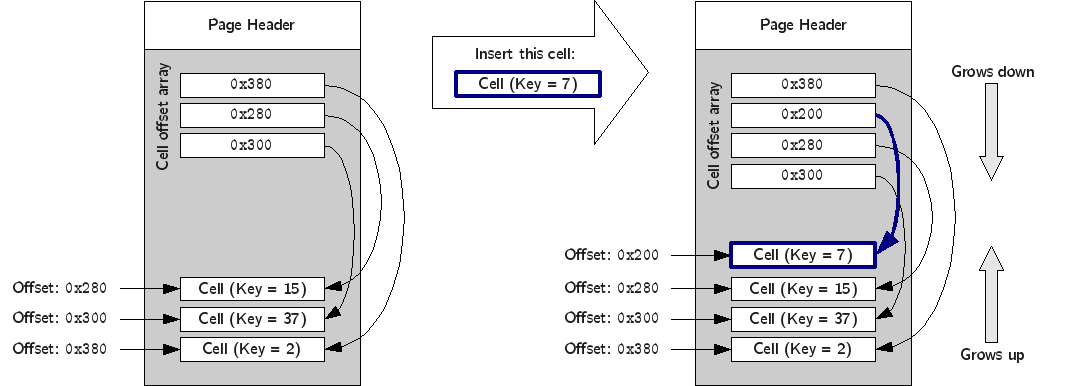
\includegraphics[width=0.8\textwidth]{images/cellsexample.png}
\end{center}
\caption{Example of a cell insertion.}
\label{fig:celloffsetarray}
\end{figure}

\begin{figure}
\begin{center}
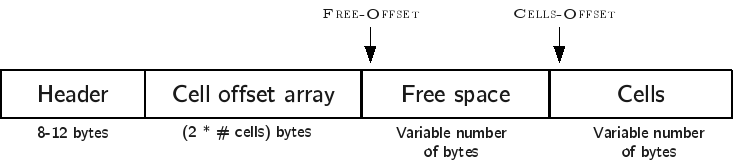
\includegraphics[width=0.4\textwidth]{images/page.png}
\end{center}
\caption{Page layout}
\label{fig:page}
\end{figure}

The exact layout of the page, summarized in Figure~\ref{fig:page} is as follows:

\begin{itemize}
\item[---] The \emph{\textbf{page header}} is located at the top of the page, and contains metadata about the page. The exact contents of the page header are explained later.
\item[---] The \emph{\textbf{cell offset array}} is located immediately after the header. Each entry is stored as a \textsf{uint16}. Thus, the length of the cell offset array depends on the number of cells in the page.
\item[---] The \emph{\textbf{cells}} are located at the end of the page.
\item[---] The space between the cell offset array and the cells is \emph{\textbf{free space}} for the cell offset array to grow (down) and the cells to grow (up). 
\end{itemize}

The layout and contents of the page header are summarized in Figure~\ref{fig:pageheader}.

\begin{figure}
\begin{center}
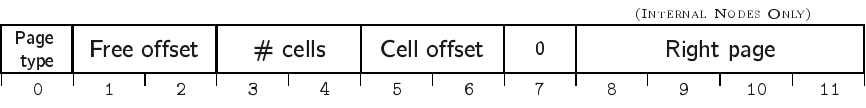
\includegraphics[width=0.7\textwidth]{images/pageheader.png}

\vspace{2em}

\sffamily
\begin{tabular}{|c|c|c|p{7cm}|}
\hline \textbf{Bytes} & \textbf{Name} & \textbf{Type} & {\centering \textbf{Description}} \\ \hline\hline
0 & \textsc{Page--Type} & \textsf{uint8} & The type of page. Valid values are \texttt{0x05} (internal table page), \texttt{0x0D} (leaf table page), \texttt{0x02} (internal index page), and \texttt{0x0A} (leaf index page) \\ \hline
1-2 & \textsc{Free--Offset} & \textsf{uint16} & The byte offset at which the free space starts. Note that this must be updated every time the cell offset array grows. \\ \hline
3-4 & \textsc{N--Cells} & \textsf{uint16} & The number of cells stored in this page. \\ \hline
5-6 & \textsc{Cells--Offset} & \textsf{uint16} & The byte offset at which the cells start. If the page contains no cells, this field contains the value \textsc{Page--Size}. This value must be updated every time a cell is added. \\ \hline
8-11 & \textsc{Right--Page} & \textsf{uint32} & See Section~\ref{sec:physorg} for a description of this value. \\ \hline
\end{tabular}
\caption{Page header}
\label{fig:pageheader}
\end{center}
\end{figure}


\section{Table cells}
\label{sec:tablecells}

The layout and contents of internal and leaf table cells are summarized in Figures~\ref{fig:tableinternalcell} and \ref{fig:tableleafcell}, respectively.

\begin{figure}
\begin{center}
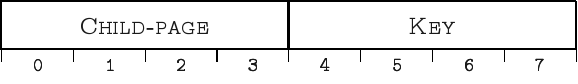
\includegraphics[width=0.4\textwidth]{images/table_internalcell.png}

\vspace{2em}

\sffamily
\begin{tabular}{|c|c|c|p{7cm}|}
\hline \textbf{Bytes} & \textbf{Name} & \textbf{Type} & {\centering \textbf{Description}} \\ \hline\hline
0-3 & \textsc{Child--Page} & \textsf{uint32} & As defined in Section~\ref{sec:physorg} \\ \hline
4-7 & \textsc{Key} & \textsf{varint32} & As defined in Section~\ref{sec:physorg} \\ \hline
\end{tabular}
\end{center}
\caption{Internal cell (table)}
\label{fig:tableinternalcell}
\end{figure}


\begin{figure}
\begin{center}
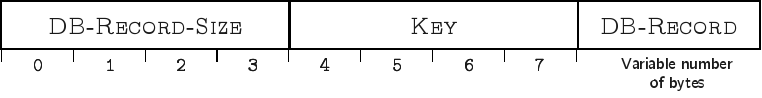
\includegraphics[width=0.6\textwidth]{images/table_leafcell.png}

\vspace{2em}

\sffamily
\begin{tabular}{|c|c|c|p{7cm}|}
\hline \textbf{Bytes} & \textbf{Name} & \textbf{Type} & {\centering \textbf{Description}} \\ \hline\hline
0-3 & \textsc{DB--Record--Size} & \textsf{varint32} & Length of \textsc{DB--Record} in bytes. \\ \hline
4-7 & \textsc{Key} & \textsf{varint32} & As defined in Section~\ref{sec:physorg} \\ \hline
8-\ldots & \textsc{DB--Record} & See Section~\ref{sec:records} & As defined in Section~\ref{sec:physorg} \\ \hline
\end{tabular}
\end{center}
\caption{Leaf cell (table)}
\label{fig:tableleafcell}
\end{figure}

\section{Database records}
\label{sec:records}

A database record is used to store the contents of a single table tuple (or ``row''). It can contain a variable number of values of NULL, integer, or text types. The record is divided into two parts: the record header and the record data. The record header specifies the types of the values contained in the record. However, the header does not include schema information. In other word, a record header may specify that the record contains an integer, followed by a string, followed by null value, followed by an integer, but does not store the names of the fields, as given when the table was created (this information is stored in the schema table, described in Section~\ref{sec:schema}). However, values in a database record must be stored in the same order as specified in the \texttt{CREATE TABLE} statement used to create the table.

The format of a database record is shown in Figure~\ref{fig:record}. The header's first byte is used to store the length in bytes of the header (including this first byte). This is followed by $n$ \textsf{varint8}s or \textsf{varint32}s, where $n$ is the number of values stored in the record. The supported types are listed in Table~\ref{tab:sqltypes}. A \textsf{varint8} is used to specify types \texttt{NULL}, \texttt{BYTE}, \texttt{SMALLINT}, and \texttt{INTEGER}, while a \textsf{varint32} is used to specify a \texttt{TEXT} type. 

\begin{figure}
\begin{center}
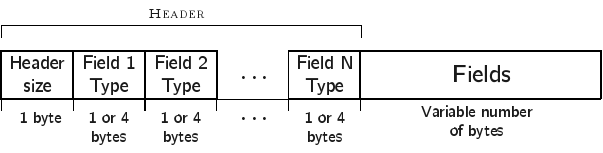
\includegraphics[width=0.6\textwidth]{images/record.png}
\end{center}
\caption{Database record format}
\label{fig:record}
\end{figure}

\begin{table}
\caption{SQL types}
\begin{center}
\sffamily
\begin{tabular}{|c|c|c|p{7cm}|}
\hline \textbf{Header value} & \textbf{SQL type} & \textbf{Internal type used in record data} \\ \hline\hline
0 & \texttt{NULL} & N/A  \\ \hline
1 & \texttt{BYTE} & \textsf{int8} \\ \hline
2 & \texttt{SMALLINT} & \textsf{int16} \\ \hline
4 & \texttt{INTEGER} & \textsf{int32} \\ \hline
$2\cdot n + 13$ & \texttt{TEXT} & \textsf{raw-string($n$)} \\ \hline
\end{tabular}
\end{center}
\label{tab:sqltypes}
\end{table}


The record data contains the actual values, in the same order as specified in the header. Note that a value of type \texttt{NULL} is not actually stored in the record data (it just has to be specified in the header). Additionally, the value that corresponds to the table's primary key is always stored as a \texttt{NULL} value (since it is already stored as the key of the B-Tree cell where the record is stored, repeating it in the record would be redundant). Figure~\ref{fig:recordexample} shows an example of how a record would be encoded internally.

\begin{figure}
\begin{center}
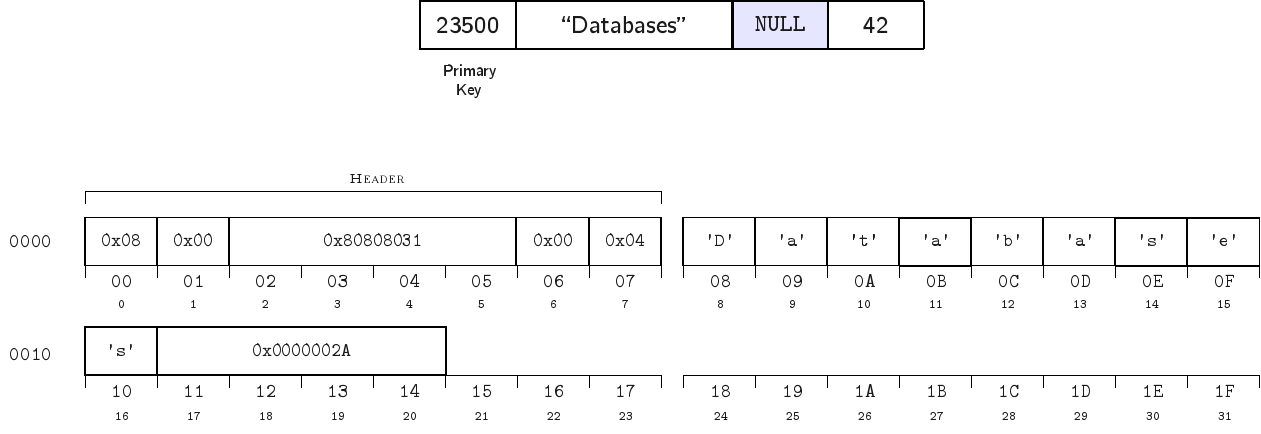
\includegraphics[width=\textwidth]{images/recordexample.png}
\end{center}
\caption{Database record example, for a table created with \texttt{CREATE TABLE Courses(Id INTEGER PRIMARY KEY, Name TEXT, Instructor INTEGER, Dept INTEGER)} }
\label{fig:recordexample}
\end{figure}





\section{Indexes}
\label{sec:indexes}

An index B-Tree is very similar to a table B-Tree, so most of what was discussed in the previous sections is applicable to indexes. The main differences are the following:

\begin{itemize}
\item[---] \textsc{Page--Type} field of the page header must be set to the appropriate value (\texttt{0x02} for internal pages and \texttt{0x0A} for leaf pages)
\item[---] While a table is stored as a B$^+$-Tree (records are only stored in the leaf nodes), an index is stored as a B-Tree (records are stored at all levels). However, an index does not store database records but, rather, $\langle \textsc{Key--Idx}, \textsc{Key--Pk} \rangle$ pairs, as defined in Section~\ref{sec:physorg}. The format of the index B-Tree cells is show in Figure~\ref{fig:indexinternalcell} (internal cells) and Figure~\ref{fig:indexleafcell}. Notice how they both differ only in the \textsc{Child--Page} field.
\end{itemize}

\begin{figure}
\begin{center}
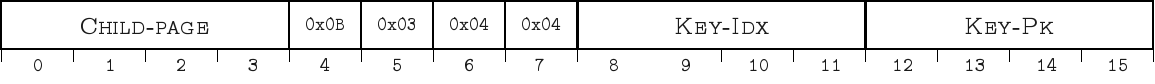
\includegraphics[width=0.8\textwidth]{images/index_internalcell.png}

\vspace{2em}

\sffamily
\begin{tabular}{|c|c|c|p{7cm}|}
\hline \textbf{Bytes} & \textbf{Name} & \textbf{Type} & {\centering \textbf{Description}} \\ \hline\hline
0-3 & \textsc{Child--Page} & \textsf{uint32} & As defined in Section~\ref{sec:physorg} \\ \hline
8-11 & \textsc{Key--Idx} & \textsf{uint32} & As defined in Section~\ref{sec:physorg} \\ \hline
12-15 & \textsc{Key--Pk} & \textsf{uint32} & As defined in Section~\ref{sec:physorg} \\ \hline
\end{tabular}
\end{center}
\caption{Internal cell (index)}
\label{fig:indexinternalcell}
\end{figure}


\begin{figure}
\begin{center}
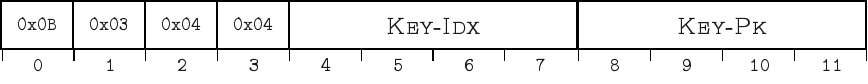
\includegraphics[width=0.6\textwidth]{images/index_leafcell.png}

\vspace{2em}

\sffamily
\begin{tabular}{|c|c|c|p{7cm}|}
\hline \textbf{Bytes} & \textbf{Name} & \textbf{Type} & {\centering \textbf{Description}} \\ \hline\hline
4-7 & \textsc{Key--Idx} & \textsf{uint32}  & As defined in Section~\ref{sec:physorg}  \\ \hline
8-11 & \textsc{Key--Pk} & \textsf{uint32} & As defined in Section~\ref{sec:physorg} \\ \hline
\end{tabular}
\end{center}
\caption{Leaf cell (index)}
\label{fig:indexleafcell}
\end{figure}


\section{The schema table}
\label{sec:schema}

Up to this point, this document has covered how to store one or more tables and indexes in a \chidb{} file. However, there is no way of knowing how many tables/indexes are stored in the file, what their schema is, and how the indexes relate to the tables. This information is stored in a special \emph{schema table}. More specifically, a \chidb{} file will always contain at least one table B-Tree, rooted in page 1, which will be used to store information on the database schema. The schema table contains one record for each table and index in the database. Table~\ref{tab:schemafields} lists the values that must be stored in each record. 

\begin{table}
\caption{Fields of a schema table record}
\begin{center}
\sffamily
\begin{tabular}{|c|c|p{7cm}|}
\hline \textbf{Type} & \textbf{Name} & \textbf{Description} \\ \hline\hline
\texttt{TEXT} & Schema item type & \texttt{table} or \texttt{index}  \\ \hline
\texttt{TEXT} & Schema item name & Name of the table or index as specified in the \texttt{CREATE TABLE} or \texttt{CREATE INDEX} statement. \\ \hline
\texttt{TEXT} & Associated table name & For tables, this field is the same as the schema item name (the name of the table). For indexes, this value contains the name of the indexed table. \\ \hline
\texttt{INTEGER} & Root page & Database page where the root node of the B-Tree is stored. \\ \hline
\texttt{TEXT} & SQL statement & The SQL statement used to create the table or index. \\ \hline
\end{tabular}
\end{center}
\label{tab:schemafields}
\end{table}

\begin{table}
\caption{Example of a schema table}
\begin{center}
\sffamily
\begin{tabular}{|c|c|c|c|p{7cm}|}
\hline \textbf{Type} & \textbf{Name} & \textbf{Assoc. Table} & \textbf{Root Page} & \textbf{SQL} \\ \hline\hline
table & Courses & Courses & 2 & \texttt{CREATE TABLE Courses(Id INTEGER PRIMARY KEY, Name TEXT, Instructor INTEGER, Dept INTEGER)}   \\ \hline
table & Instructors & Instructors & 3 & \texttt{CREATE TABLE Instructors(Id INTEGER PRIMARY KEY, Name TEXT)}   \\ \hline
index & idxInstr & Courses & 6 & \texttt{CREATE INDEX idxInst ON Courses(Instructor)}   \\ \hline
\end{tabular}
\end{center}
\label{tab:schemaexample}
\end{table}

\section{Copyright information}

This work is licensed under the Creative Commons Attribution-Share Alike 3.0 United States License. To view a copy of this license, visit http://creativecommons.org/licenses/by-sa/3.0/us/ or send a letter to Creative Commons, 171 Second Street, Suite 300, San Francisco, California, 94105, USA.


\end{document}
